%% Beamer slides: Towards a Cartography of Datacentering
%% Research Policy 11th Online ECR Conference, 27 April 2026
%% Theme: Metropolis

\documentclass[aspectratio=169,12pt]{beamer}

\usetheme{metropolis}
\usepackage{booktabs}
\usepackage{tabularx}
\usepackage{array}
\usepackage{tikz}
\usetikzlibrary{arrows.meta,positioning,shapes.geometric,fit,backgrounds}

%% Metropolis colour overrides
\definecolor{dcblue}{RGB}{31,73,125}
\definecolor{dcaccent}{RGB}{192,80,77}
\definecolor{dclightblue}{RGB}{189,215,238}
\definecolor{dcgray}{RGB}{89,89,89}

\setbeamercolor{frametitle}{bg=dcblue,fg=white}
\setbeamercolor{progress bar}{fg=dcaccent}
\setbeamercolor{alerted text}{fg=dcaccent}
\setbeamercolor{example text}{fg=dcblue}

\title{Towards a Cartography of Datacentering}
\subtitle{A Multimodal Research Agenda}
\author{Babajide Owoyele}
\institute{Erasmus University Rotterdam}
\date{Research Policy ECR Conference \\ 27 April 2026}

%% ------------------------------------------------------------------
\begin{document}

%% SLIDE 1 — Title
\maketitle

%% ------------------------------------------------------------------
%% SLIDE 2 — The Empirical Provocation
\begin{frame}{The Empirical Provocation}
\begin{columns}[T]
\begin{column}{0.5\textwidth}
  \textbf{4,757 papers on data centers} (OpenAlex, 2010--2025)\\[0.4em]
  Growth: \alert{372\%} in 15 years\\[0.6em]

  \begin{tabular}{lr}
  \toprule
  Silo & Papers \\
  \midrule
  Technical efficiency & $\approx 279$ \\
  Environmental impact & $\approx 114$ \\
  Socio-political      & $\approx 15$  \\
  \midrule
  \alert{Innovation studies} & \alert{0} \\
  \bottomrule
  \end{tabular}
\end{column}
\begin{column}{0.46\textwidth}
  \vspace{0.2em}
  \begin{center}
  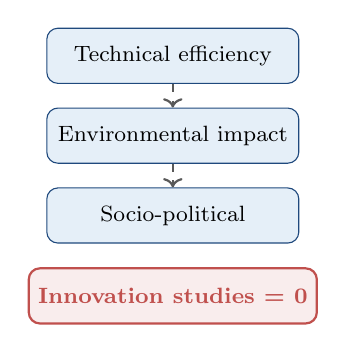
\begin{tikzpicture}[scale=0.82,every node/.style={font=\footnotesize}]
    \node[draw=dcblue,fill=dclightblue!40,rounded corners,
          minimum width=3.2cm,minimum height=0.7cm,
          text centered] (s1) {Technical efficiency};
    \node[draw=dcblue,fill=dclightblue!40,rounded corners,
          minimum width=3.2cm,minimum height=0.7cm,
          text centered,below=0.3cm of s1] (s2) {Environmental impact};
    \node[draw=dcblue,fill=dclightblue!40,rounded corners,
          minimum width=3.2cm,minimum height=0.7cm,
          text centered,below=0.3cm of s2] (s3) {Socio-political};
    \node[draw=dcaccent,thick,fill=dcaccent!10,rounded corners,
          minimum width=3.2cm,minimum height=0.7cm,
          text centered,text=dcaccent,
          font=\footnotesize\bfseries,below=0.3cm of s3] (s4)
          {Innovation studies = 0};
    \draw[->,thick,dcgray,dashed] (s1) -- (s2);
    \draw[->,thick,dcgray,dashed] (s2) -- (s3);
  \end{tikzpicture}
  \end{center}
\end{column}
\end{columns}
\end{frame}

%% ------------------------------------------------------------------
%% SLIDE 3 — What the Cloud Conceals
\begin{frame}{What ``The Cloud'' Conceals}
\begin{columns}[T]
\begin{column}{0.55\textwidth}
  The word \alert{``cloud''} does ideological work:\\[0.4em]
  \begin{itemize}
    \item Naturalises infrastructure — makes it weightless, placeless
    \item Conceals: water, land, power, fibre, diesel
    \item \textbf{$\approx 400$ TWh/year} globally — fastest-growing OECD electricity user
  \end{itemize}
  \vspace{0.5em}
  Make it visible and you find: actors, contestation, governance, regime change
\end{column}
\begin{column}{0.4\textwidth}
  \begin{tabular}{ll}
  \toprule
  Resource & Scale \\
  \midrule
  Electricity & 400 TWh/yr \\
  Water       & ML/day \\
  Land        & Industrial \\
  Finance     & REIT, PE, SWF \\
  \bottomrule
  \end{tabular}
\end{column}
\end{columns}
\end{frame}

%% ------------------------------------------------------------------
%% SLIDE 4 — Introducing Datacentering
\begin{frame}{Introducing ``Datacentering''}

\metroset{block=fill}
\begin{block}{Concept}
  \textbf{Datacentering} = the active socio-material process through which digital
  infrastructure is continuously assembled, contested, and reproduced
\end{block}

\vspace{0.6em}
\begin{columns}[T]
\begin{column}{0.48\textwidth}
  \textbf{Why a gerund?}
  \begin{itemize}
    \item Process over static object
    \item Who is doing the datacentering?
    \item What is being assembled or foreclosed?
  \end{itemize}
\end{column}
\begin{column}{0.48\textwidth}
  \textbf{Theoretical grounding}
  \begin{itemize}
    \item Orlikowski (2007): sociomaterial entanglement
    \item Jasanoff \& Kim (2015): imaginaries co-produce material facts
    \item ``Cloud'' suppresses what datacentering names
  \end{itemize}
\end{column}
\end{columns}
\end{frame}

%% ------------------------------------------------------------------
%% SLIDE 5 — CAS Framework
\begin{frame}{Theoretical Framework: CAS as Sensemaking Lens}

\begin{center}
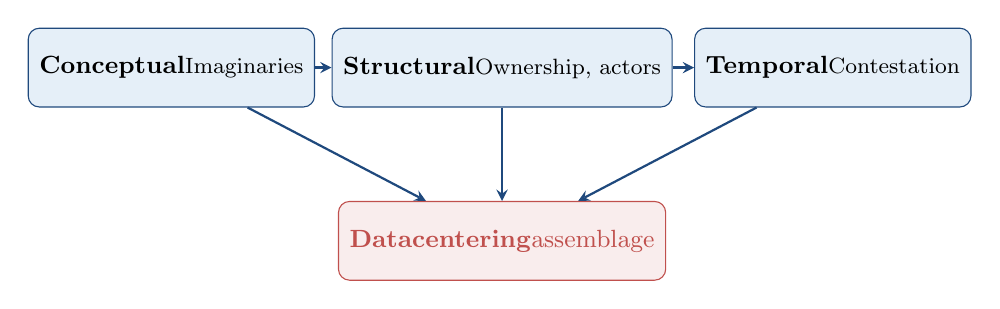
\begin{tikzpicture}[
  box/.style={draw=dcblue,fill=dclightblue!40,rounded corners,
              minimum width=3.0cm,minimum height=1.0cm,
              text centered,font=\small,inner sep=4pt},
  arr/.style={->,>=stealth,thick,dcblue}
]
  \node[box] (c) at (0,0)   {\textbf{Conceptual}\newline{\footnotesize Imaginaries}};
  \node[box] (s) at (4.2,0) {\textbf{Structural}\newline{\footnotesize Ownership, actors}};
  \node[box] (t) at (8.4,0) {\textbf{Temporal}\newline{\footnotesize Contestation}};
  \node[box,draw=dcaccent,fill=dcaccent!10,text=dcaccent,font=\small] (dc)
        at (4.2,-2.2) {\textbf{Datacentering}\newline assemblage};
  \draw[arr] (c) -- (s);
  \draw[arr] (s) -- (t);
  \draw[arr] (c) -- (dc);
  \draw[arr] (s) -- (dc);
  \draw[arr] (t) -- (dc);
\end{tikzpicture}
\end{center}

\par\medskip
\begin{center}
\small After \textbf{Phillips \& Ritala (2019)} --- sensemaking lens, not a formal model\par\smallskip
Data center assemblages = \alert{multi-actor, nonlinear, emergent}
\end{center}

\end{frame}

%% ------------------------------------------------------------------
%% SLIDE 6 — Multimodal Methodology
\begin{frame}{A Multimodal Research Agenda}

\begin{center}
\begin{tabular}{llll}
\toprule
\textbf{WP} & \textbf{CAS Dimension} & \textbf{Data} & \textbf{Output} \\
\midrule
WP1 & Conceptual   & Operator websites, Wikipedia       & Imaginary divergence \\
WP2 & Conceptual   & Satellite + corporate imagery      & Abstraction score    \\
WP3 & Structural   & OpenCorporates, REIT filings       & Ownership network    \\
WP4 & Temporal     & News, planning records, social media & Signal-to-response lag \\
\bottomrule
\end{tabular}
\end{center}

\vspace{0.5em}
\metroset{block=fill}
\begin{block}{Why multimodal?}
  Strategic opacity is a \textit{sociotechnical fact} — not a data gap.\\
  \small A firm that won't publish is still in a REIT filing, a Sentinel-2 image, and a planning record.
\end{block}

\end{frame}

%% ------------------------------------------------------------------
%% SLIDE 7 — WP1 + WP2
\begin{frame}{WP1 \& WP2: The Conceptual Dimension}
\begin{columns}[T]
\begin{column}{0.48\textwidth}
  \metroset{block=fill}
  \begin{block}{WP1 — Territorial Imaginaries}
    \begin{itemize}
      \item Corporate websites vs.\ city Wikipedia
      \item Keyword asymmetry diagnostic
      \item \textbf{ECI divergence score}
      \item High sustainability / low community\\= placelessness production
    \end{itemize}
  \end{block}
\end{column}
\begin{column}{0.48\textwidth}
  \metroset{block=fill}
  \begin{block}{WP2 — Strategic Invisibility}
    \begin{itemize}
      \item Sentinel-2 satellite imagery
      \item Corporate photography (CLIP)
      \item \textbf{Visual abstraction score}
      \item Abstract imagery performs\\the cloud imaginary
    \end{itemize}
  \end{block}
\end{column}
\end{columns}
\vspace{0.6em}
\begin{center}
  \textit{How do actors construct imaginaries that make datacentering \textbf{legible or illegible}?}
\end{center}
\end{frame}

%% ------------------------------------------------------------------
%% SLIDE 8 — WP3 + WP4
\begin{frame}{WP3 \& WP4: Structural and Temporal Dimensions}
\begin{columns}[T]
\begin{column}{0.48\textwidth}
  \metroset{block=fill}
  \begin{block}{WP3 — Ownership Cartography}
    \begin{itemize}
      \item OpenCorporates + REIT filings
      \item \textbf{REIT structure} disperses accountability
      \item Ownership network + actor typology
    \end{itemize}
  \end{block}
\end{column}
\begin{column}{0.48\textwidth}
  \metroset{block=fill}
  \begin{block}{WP4 — Contestation Signals}
    \begin{itemize}
      \item News archives, planning records
      \item BERTopic + event detection
      \item \textbf{Signal-to-response lag}
    \end{itemize}
  \end{block}
\end{column}
\end{columns}
\vspace{0.6em}
\begin{center}
  \textit{Who does the datacentering, in what legal form, and what happens when communities resist?}
\end{center}
\end{frame}

%% ------------------------------------------------------------------
%% SLIDE 9 — Virginia vs Amsterdam
\begin{frame}{Illustrative Comparison: Virginia vs Amsterdam}
\begin{center}
\begin{tabular}{lll}
\toprule
\textbf{Dimension} & \textbf{Northern Virginia} & \textbf{Amsterdam} \\
\midrule
Ownership          & REIT-dominated, dispersed  & Mixed; operator-owned, cooperative \\
Governance counterparty & None identifiable     & Municipality + named operators \\
Territorial imaginary   & Placeless            & Contested, partially negotiated \\
Contestation intensity  & \alert{High}         & \alert{High} \\
Regime response         & \textbf{None}        & \textbf{Moratorium 2019--2022} \\
\midrule
\textbf{Key variable} & \multicolumn{2}{l}{Not signal strength — \alert{regime structure}} \\
\bottomrule
\end{tabular}
\end{center}
\vspace{0.3em}
\begin{center}
  \small This is the question MLP was built to answer — and the existing literature cannot.
\end{center}
\end{frame}

%% ------------------------------------------------------------------
%% SLIDE 10 — Open Cartography Invitation
\begin{frame}{Building the Cartography Together}
\begin{columns}[T]
\begin{column}{0.55\textwidth}
  \textbf{Why open exchange is a theoretical necessity}\\[0.4em]
  Datacentering is CAS-like: too large, too distributed, too opaque for any single team.\\[0.4em]
  The research commons is the methodological response to the complexity of the object.\\[0.6em]
  \textbf{What we are sharing:}
  \begin{itemize}
    \item Community facility index (CC BY 4.0)
    \item NLP / CV / network pipelines (MIT)
    \item Open data, open workflows
  \end{itemize}
\end{column}
\begin{column}{0.42\textwidth}
  \textbf{Concrete asks:}
  \begin{itemize}
    \item Local knowledge of disputes, moratoriums, unreported facilities
    \item National company registry or REIT data access
    \item Methodological critique
    \item Replication in other languages
  \end{itemize}
\end{column}
\end{columns}
\vspace{0.5em}
\begin{center}
  \large\textit{The cloud is not a metaphor. It is infrastructure.\\And infrastructure can be mapped.}
\end{center}
\end{frame}

\end{document}
